{Two blocks of masses $m_1$ and $m_2$ are connected by a string over a smooth pulley as shown.  Assume that $m_2>m_1$.  If the coefficient of friction is $\mu$ and $r=m_1/m_2$, then the masses will move at a constant speed ($m_2$ slides down the slope) if the angle $\theta$ is given by $\displaystyle \cos(\theta) = \frac{-\mu r + \sqrt{1-r^2+\mu^2}}{1+\mu^2}$.

%\begin{center}
%\includegraphics[scale=.3]{figures/matlab_ramp.png}
%\end{center}

\begin{center}
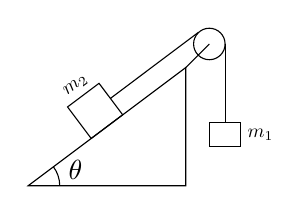
\begin{tikzpicture}[scale=1]

\draw (0,0) node [shift={(.6,.2)},scale=1] {$\theta$} -- (2,0) -- (2,1.5) -- cycle; % angle is 36.86989765 degrees
\draw (.4,0) arc (0:36.9:.4);
\draw (2,1.5) -- ++(.3,.3) circle (.2);
\draw [rotate=36.9](1,0) -- (1.5,0) -- (1.5,.5) -- node [pos=.5,rotate=36.9,scale=.7,above] {$m_2$} (1,.5)--cycle (1.5,.26) -- (2.9,.26);
\draw (2.5,1.8) -- (2.5,.8);
\draw (2.3,.8) -- (2.7,.8) -- node [pos=.5,scale=.7,right] {$m_1$} (2.7,.5) -- (2.3,.5) -- cycle;

\end{tikzpicture}
\end{center}

\begin{itemize}
\item[a.] Compute the values of the angle $\theta$ if $m_2$ is twice the value of $m_1$ and $\mu$ ranges from 0 to 1 in increments of 0.1.
\item[b.] Compute the values of the angle $\theta$ if $m_2$ is ten times the value of $m_1$ and $\mu$ ranges from 0 to 1 in increments of 0.1.
\item[c.] What can you say if $m_1=m_2$?
\end{itemize}
}{}
%http://en.wikipedia.org/wiki/Elastic_collision



%Old Problem:
%{A sphere of mass $m_1$ strikes a stationary sphere of mass $m_2$, the direction of the blow making an angle $\alpha$ with the line of motion.  If the coefficient of restitution is $e$ (i.e. ``bounciness''), it can be shown that the striking sphere is deflected through an angle $\beta$ such that
%\[
%\tan \beta=\frac{m_2(1+e)\tan \alpha}{m_1-e\, m_2+(m_1 + m_2)\tan^2 \alpha}
%\]
%Find $\beta$ if $m_1=10, m_2=5, e=1$ and $\alpha$ ranges from $30^\circ$ to $90^\circ$ (in $5^\circ$ increments).  Make sure to define the variables $m1,m2,e$ and $\alpha$ first and then define $\beta$ in terms of them.}
%{}
%